% =============================================================================
% Chapter 3 — Methodology
% =============================================================================

\chapter{Methodology: A Systematic Mapping of the Literature on Algorithmisation, 1990–2025}
\label{ch:methodology}

\section{Review Design}
\label{sec:review-design}

To empirically investigate the intersection of algorithmic governance, urban space, and systemic spatial destruction (domicide), this dissertation employed a Systematic Literature Review (SLR). Where a traditional narrative review risks selection bias by design — the `cherry-picking' of sources to validate a pre-existing critique — the SLR provides a transparent, auditable, and reproducible mechanism for data collection. This aligns with the `evidence turn' in contemporary public policy and management, which increasingly demands structured methodologies to track policy evolution and evaluate `what works' \parencite{tranfield2003}. Rather than evaluating the effectiveness of a specific policy intervention, however, the review was adapted to rigorously map a longitudinal discursive shift: how global academic discourse and policy literature conceptualised algorithms, big data, and spatial surveillance over three and a half decades.

The legitimacy of this design rests on an established methodological lineage. Developed in the health sciences, the SLR's protocol-driven design converts the literature review from an essayistic exercise into an auditable instrument: explicit search strings, pre-registered inclusion criteria, and logged screening decisions make the reviewer's judgements visible and reproducible \parencite{sutton2019}. Within Sutton and colleagues' taxonomy of the `review family', this is a \emph{mapping} review: it trades depth for breadth, charting the structure and distribution of a heterogeneous literature — exactly the analytical object this dissertation requires, since its claims concern the \emph{configuration} of a field rather than the pooled effect of an intervention \parencite{sutton2019}. The approach carries a direct precedent in social policy: Gurney's \citeyearpar[pp.~239--241]{gurney2023} systematic literature mapping of 213 COVID-19 housing studies demonstrates the method's value for converting an unwieldy, fast-moving policy literature into structured evidence of what the discourse has and has not registered. The present review applies the same logic to a colder question: not what the literature says, but where it has been silent.

The review was conducted between June and July 2026; every stage was logged with timestamps, record counts, and tooling versions, and is reported against the PRISMA 2020 statement \parencite{page2021} (Figure~\ref{fig:prisma}), rendering the final corpus fully auditable. The complete review archive — search records, screening verdicts, coding outputs, pipeline scripts, and the timestamped SLR log — is publicly available at \url{https://github.com/EVasiloudes/algorithmic-governance-domicide-slr}.

\section{Conceptual Scope and Research Questions}
\label{sec:conceptual-scope}

The core premise motivating the search parameters is the hypothesis that the algorithmisation of public policy possesses a dual-use nature that distinguishes it from the management of physical urban infrastructure. Where the build-out of legacy urban assets — highways, rail networks, gas terminals — requires massive capital expenditure, physical friction, and explicit geographic constraint, software operates under entirely different economic mandates: following Arrow's \citeyearpar[pp.~609--610]{arrow1962} analysis of the `information good' (developed fully in Chapter~2), a high initial cost of development but a near-zero marginal cost of reproduction and redeployment. The review was designed to test whether — and how — this phenomenon has been recognised, debated, or obfuscated in the literature.

The research questions are stated in full in Chapter~1 (§\ref{sec:research-questions}). Operationalised for the review, they required the collected literature to speak to two things at once: the dual-use nature of algorithmic technologies in urban governance, specifically in contrast to physical infrastructure (RQ1); and the shift from institutional, disciplinary management of urban space to algorithmic, modulatory control, insofar as that shift is implicated in systemic urban destruction or domicide (RQ2). These questions fixed the perimeter of the search.

\section{Search Strategy}
\label{sec:search-strategy}

\subsection{Databases and date range}

The review interrogated a 35-year chronological window, 1990–2025. This expansive range was a methodological necessity, allowing the review to track the literature across distinct technological epochs: from the early internet and the digitisation of municipal records in the 1990s, through the Big Data era of ubiquitous harvesting, to the current period defined by generative AI and autonomous systems. The window's breadth sacrifices depth at its edges — the early-1990s digitisation literature is sparse, and pre-1990 debates on automated warfare fall outside it entirely — but buys symmetric coverage of both literatures' full trajectories; the corpus's own distribution confirms the wager, with the post-2015 concentration of included records (Figure~\ref{fig:year-trends}) showing that the window captures the period in which the two vocabularies begin to converge.

Peer-reviewed literature was sourced from Web of Science and Scopus, chosen for their breadth across the social sciences, urban planning, and defence studies. Grey literature was sourced from Policy Commons, supplemented by targeted manual searches of key institutional repositories (RAND Corporation, Chatham House, Urban Displacement Project), emphasising policy documents, parliamentary records, defence white papers, and think-tank outputs addressing the dual-use implications of urban data technologies.

\begin{figure}[H]
\centering
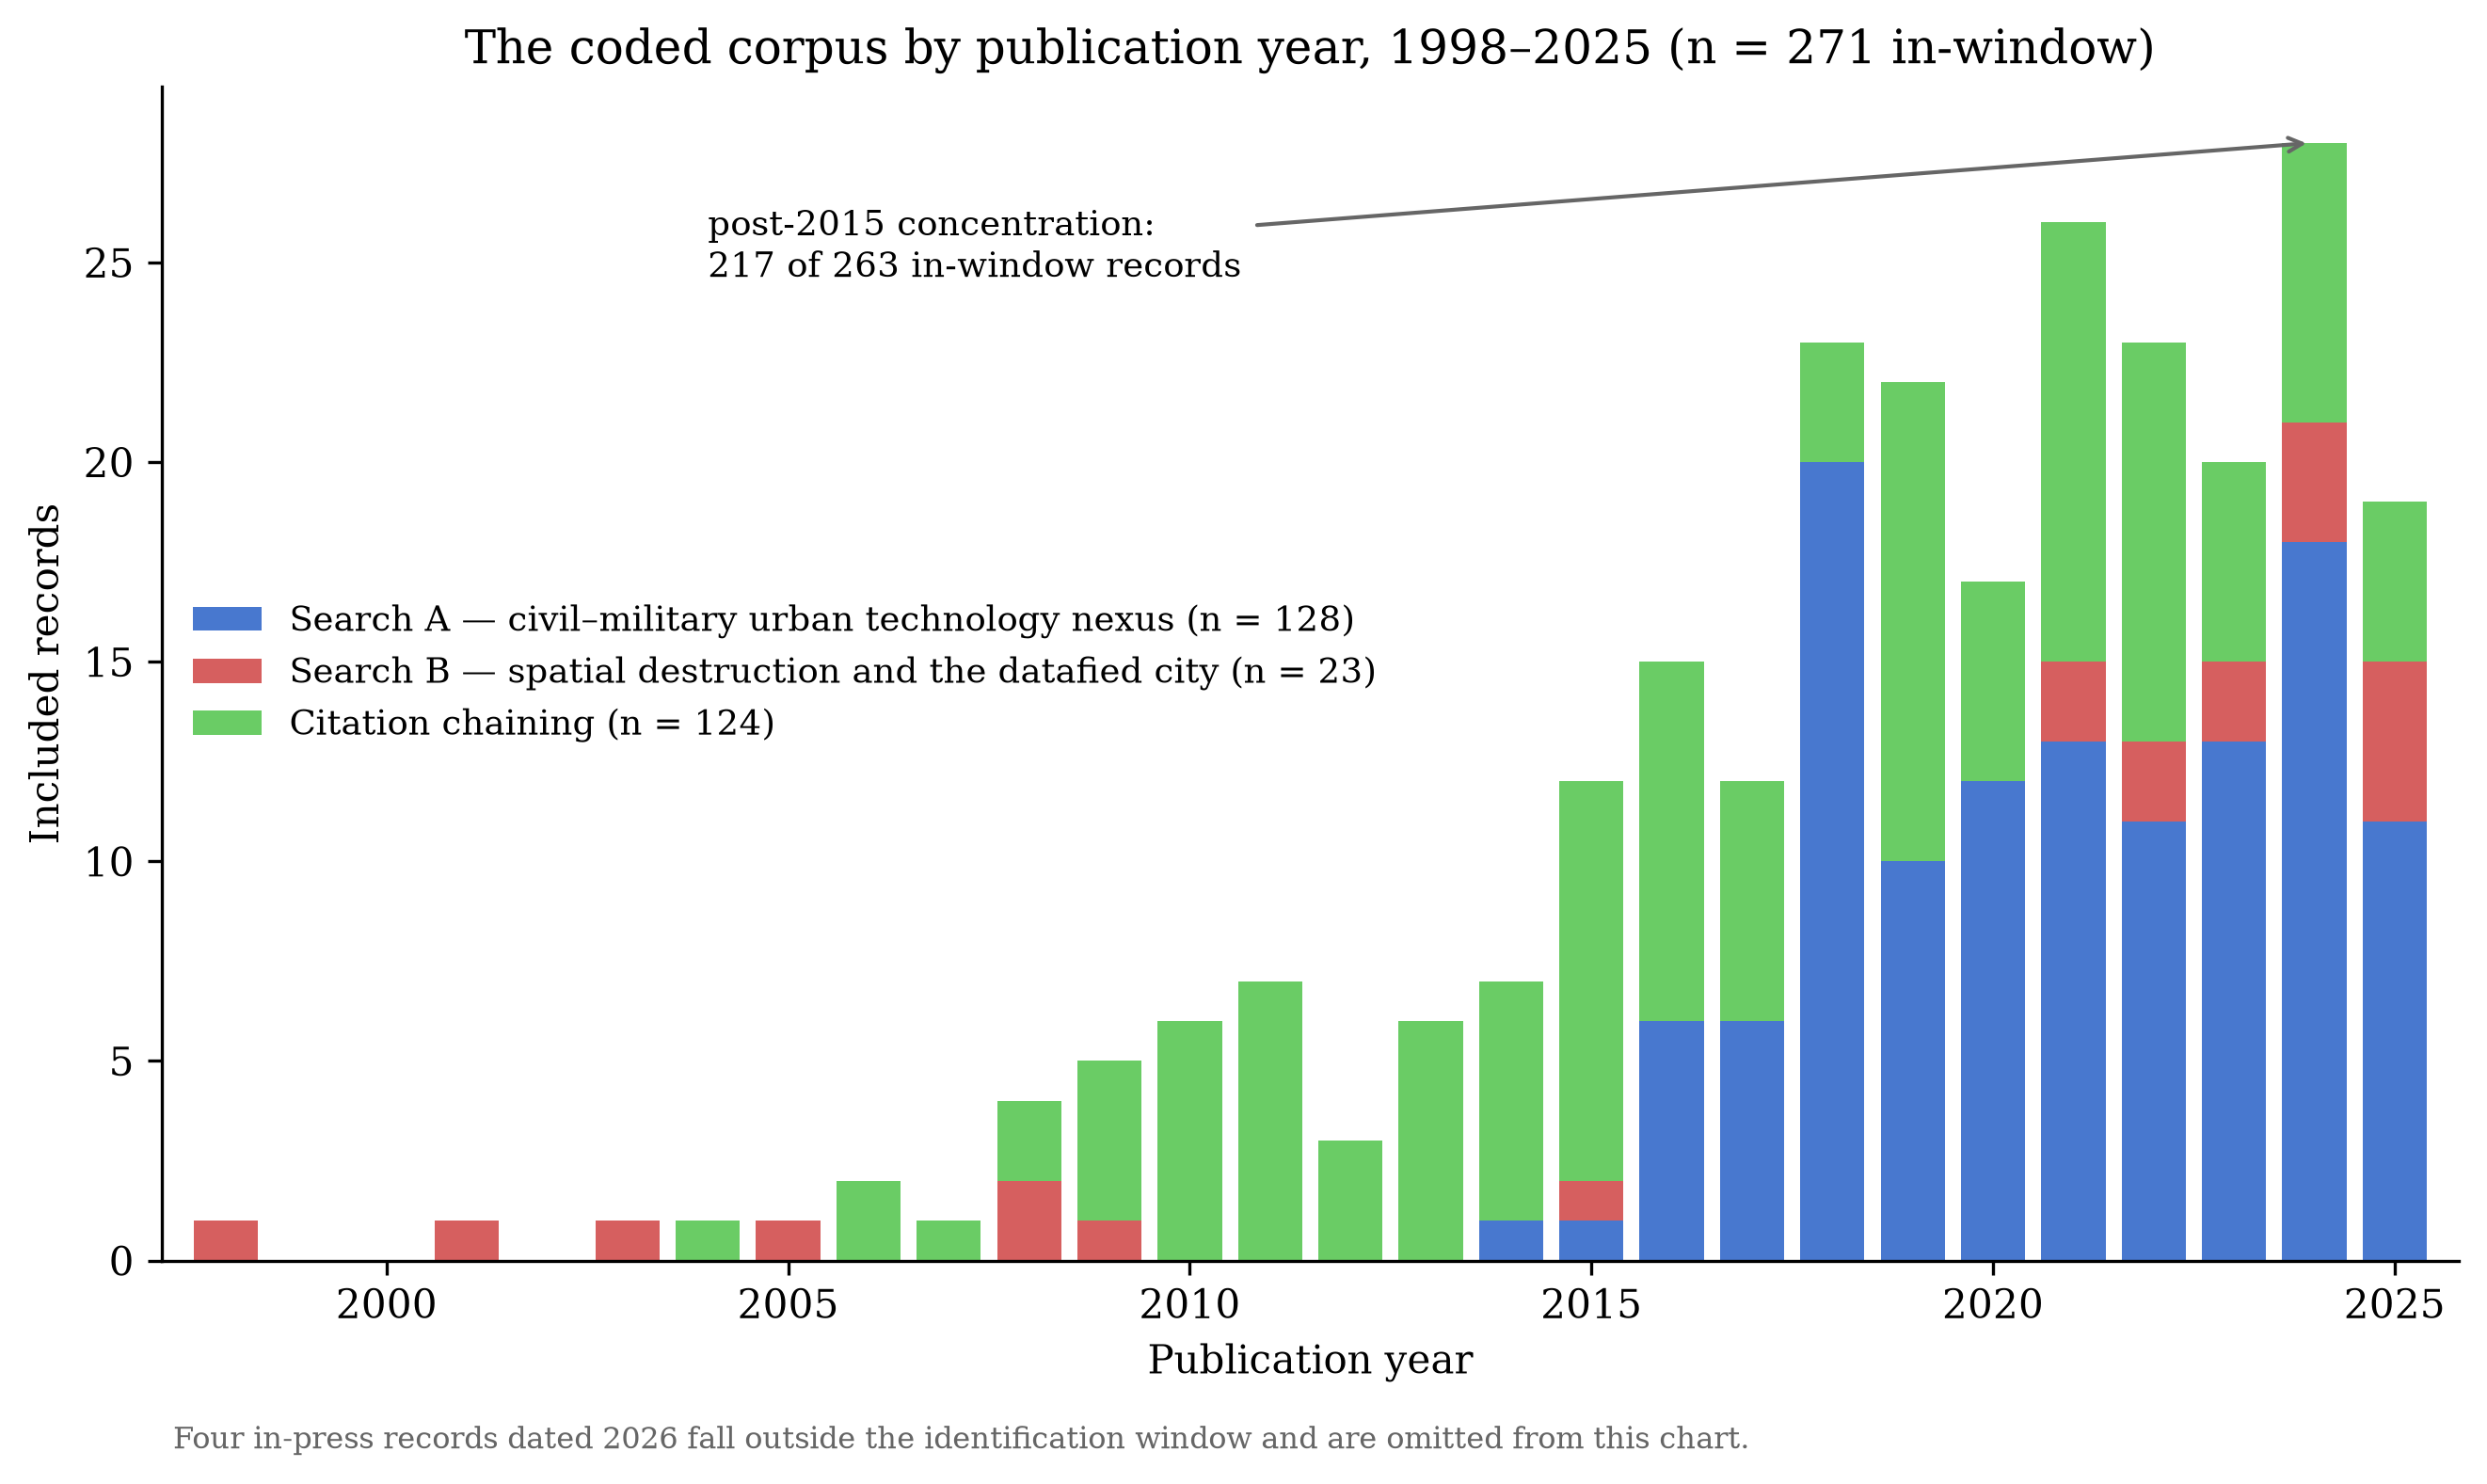
\includegraphics[width=0.95\textwidth]{figures/fig_3_2_publication_trends.png}
\caption{Publication-year distribution of the included corpus (n~=~271 in-window records), stacked by provenance. The concentration of records after 2015 --- driven by the smart-city wave on the governance side and by post-2021 work on the destruction side --- reflects the technological epochs the window was chosen to span; four in-press records dated 2026 fall outside the identification window.}
\label{fig:year-trends}
\end{figure}

The window's bookends are corroborated by field-level publication trends (Figure~\ref{fig:term-trends}): the governance vocabulary scarcely exists in the indexed literature before the mid-2000s, while the destruction vocabulary long predates the window and persists at a low, steady volume throughout it. A 1990 start therefore captures the full arc of the algorithmic-governance literature from its prehistory, and the 2025 end-point coincides with the moment the destruction literature begins to register algorithmic systems directly.

\begin{figure}[H]
\centering
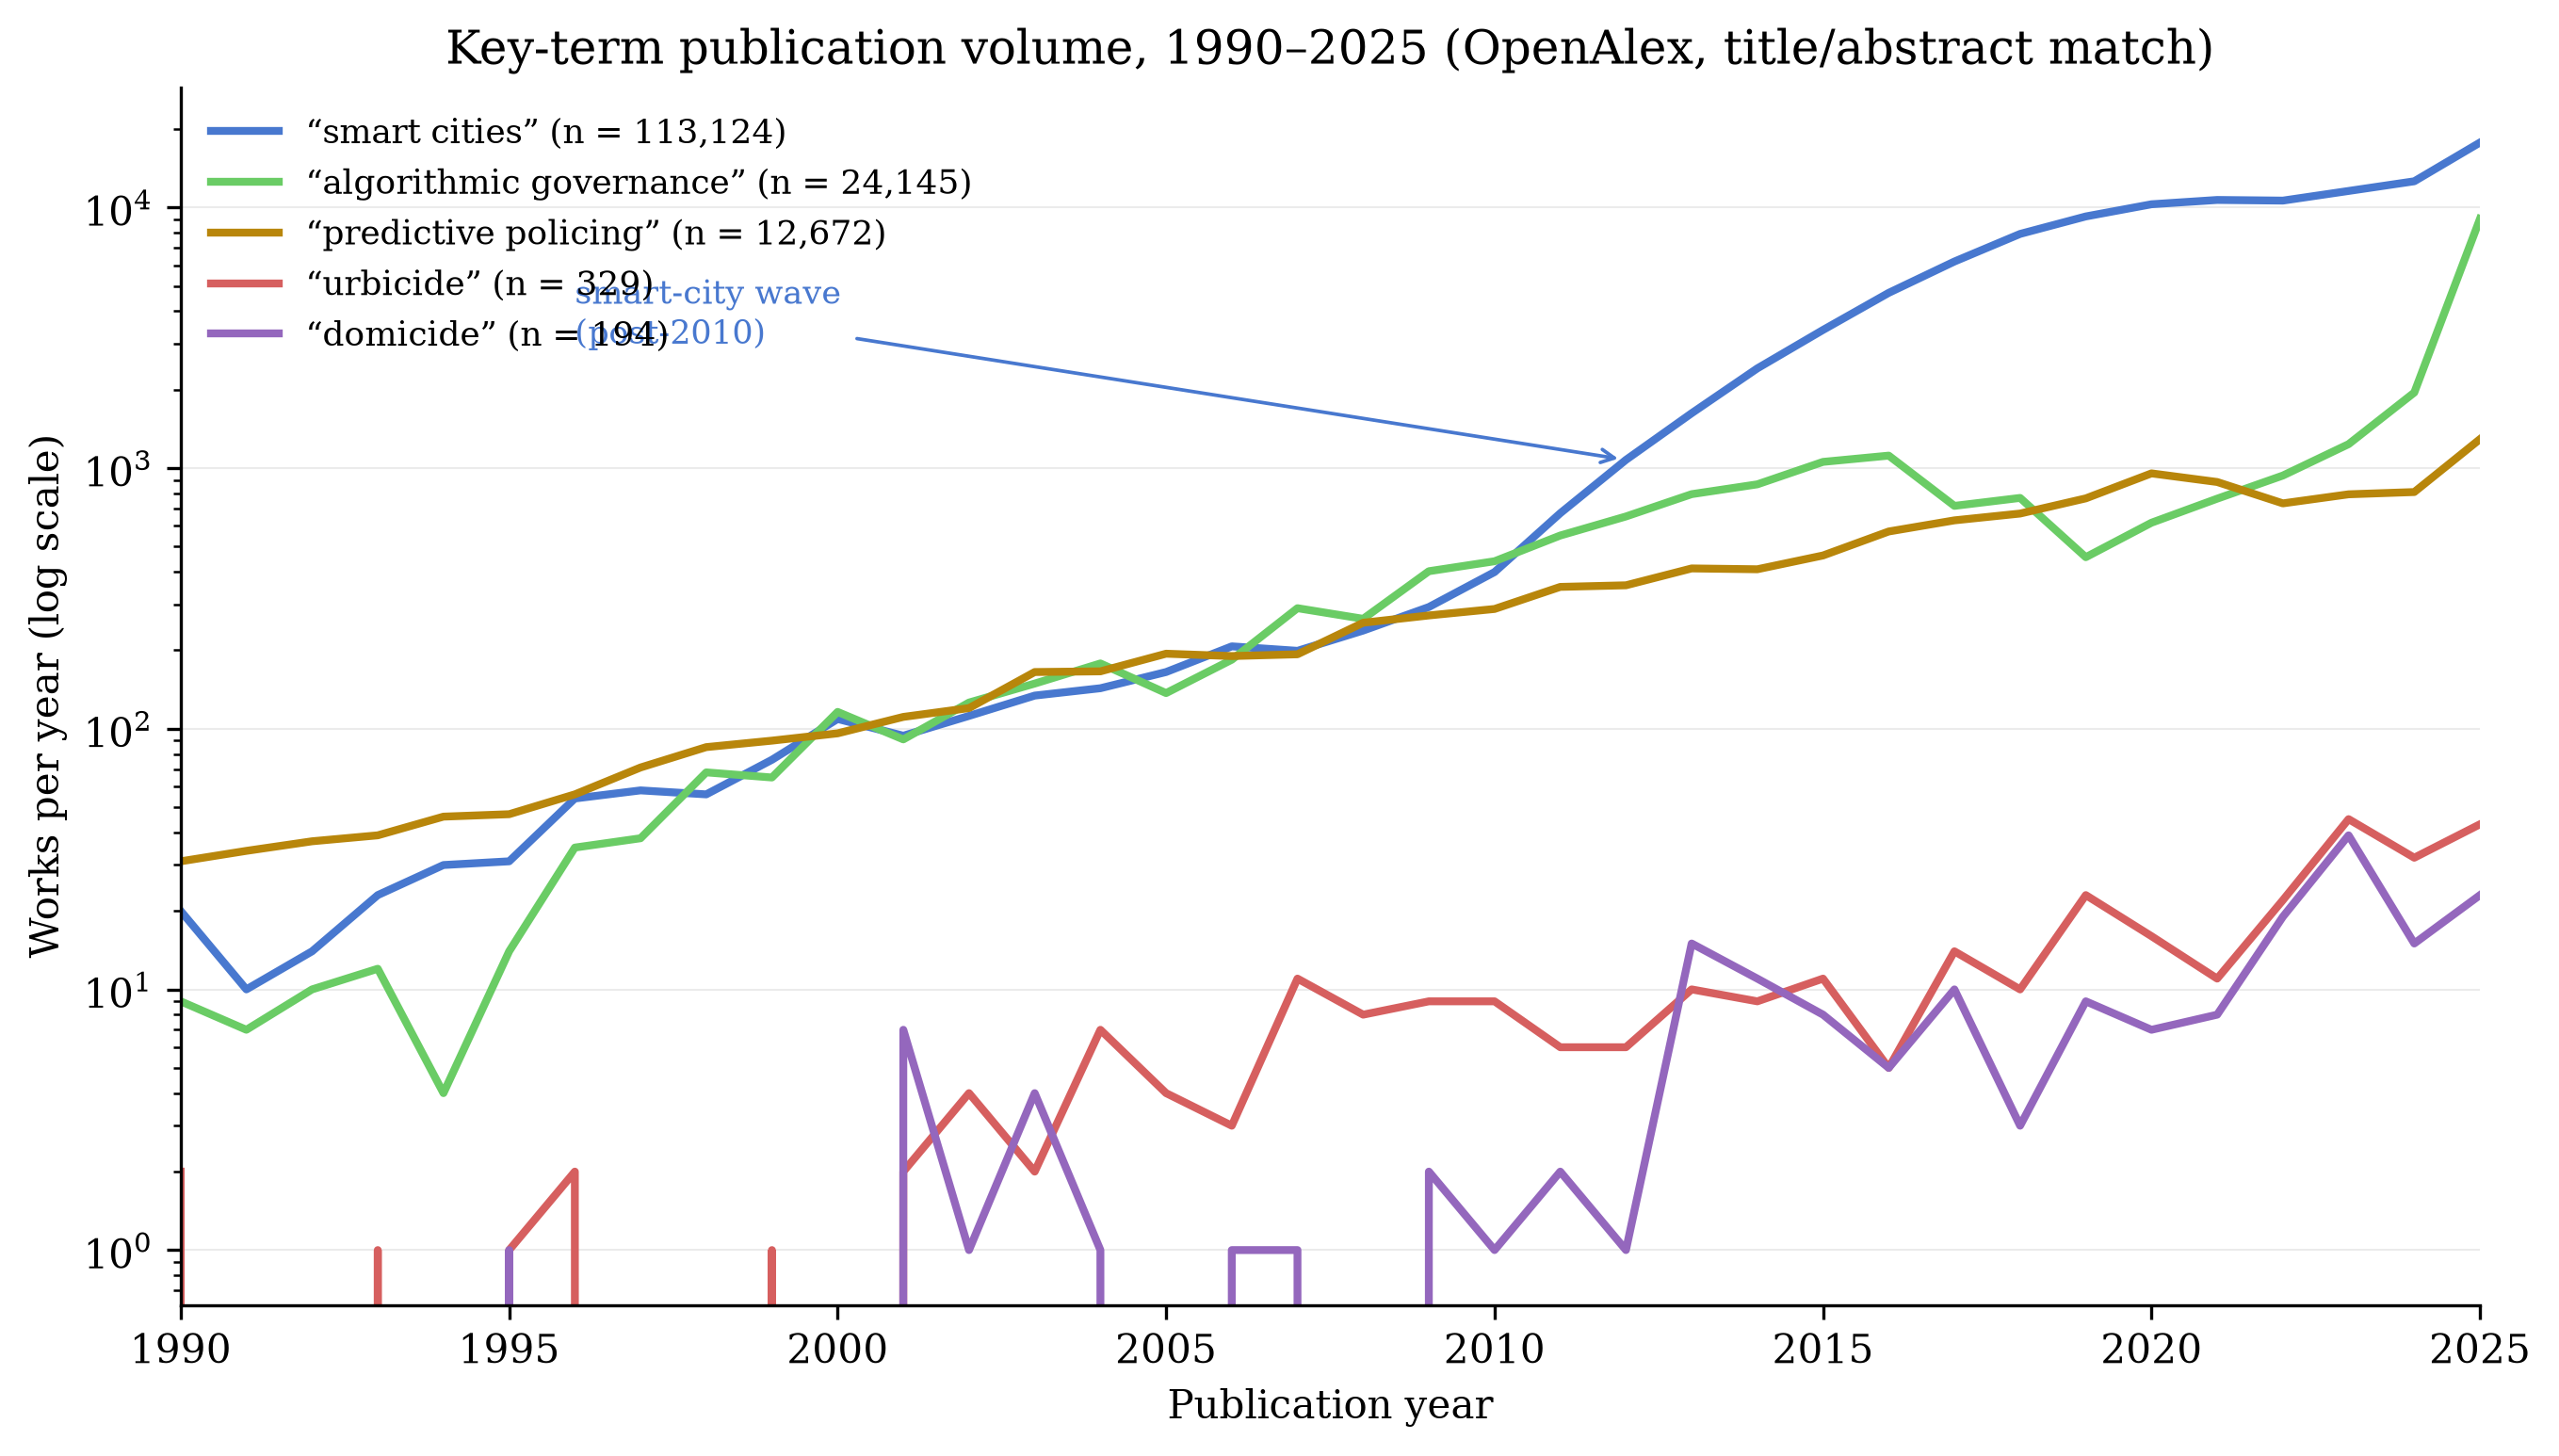
\includegraphics[width=0.95\textwidth]{figures/fig_3_3_literature_trends.png}
\caption{Publication volume for five key terms, 1990--2025, log scale (OpenAlex works matching each term in title or abstract; retrieved 6 August 2026). The governance terms (\enquote{smart cities}, \enquote{algorithmic governance}, \enquote{predictive policing}) exhibit the post-2010 spike the window was designed to capture; the destruction terms (\enquote{urbicide}, \enquote{domicide}) remain two orders of magnitude smaller, foreshadowing the asymmetry documented in Chapter~4.}
\label{fig:term-trends}
\end{figure}

\subsection{Dual-search design}

Given the cross-cutting nature of the inquiry — bridging urban analytics, security studies, and spatial destruction — a single search string risked being either too restrictive or analytically shallow. The review therefore deployed two complementary search strategies, merged at the deduplication stage.

\textbf{Search A — Civil–military urban technology nexus (high recall):} designed to surface the broader landscape of how algorithmic governance, smart city infrastructure, and urban analytics intersect with military, surveillance, and security apparatuses; the string pairs an algorithmic-governance vocabulary (``algorithmic governance'', ``urban analytics'', ``smart cit*'', ``platform urbanism'', ``predictive policing'', ``urban big data'', ``data-driven urbanism'') with a security vocabulary (``dual-use'', ``civil-military'', militari*, ``national security'', securitis*/securitiz*, weaponi*, warfare, ``state/mass surveillance'', ``OSINT'').

\textbf{Search B — Spatial destruction and the datafied city (high precision):} designed to capture literature specifically addressing how algorithmic and data-driven tools are implicated in urbicide, domicide, and spatial violence; the string pairs destruction terms (``domicide'', ``urbicide'', ``spatial violence'', ``home unmaking'', ``urban destruction'', ``urban warfare'') with data-technology terms (``data'', ``algorithm'', ``AI'', ``surveillance'', ``GIS'', ``remote sensing''). Platform-specific formulations are reproduced verbatim in Appendix~\ref{app:search}.

This dual-search approach ensured that papers theorising the surveillance–governmentality nexus (which might not explicitly invoke `domicide') and papers documenting spatial destruction (which might not deploy the language of `algorithmic governance') were both captured. The convergence — or absence of convergence — between the two literatures was itself a phenomenon the review was designed to surface.

\subsection{Calibration}

Search strings were calibrated through documented scoping iterations. An initial Scopus formulation of Search A returned 9,981 records — unmanageable for single-author screening. Diagnosis identified four generic terms driving cross-disciplinary noise — `big data', bare `security', bare `targeting', and bare `surveillance' — which were replaced with the qualified equivalents and truncated stems shown above; a date-boundary error that would have excluded 1990 and 2025 was also corrected.

Policy Commons required separate calibration. Initial strings returned 13,096 (Search A) and 3,031 (Search B) hits, owing to automatic stemming and full-text indexing across a broad grey corpus; both searches were revised to fielded formulations (Search A: both legs in the summary field; Search B: spatial-destruction terms in title, data terms in summary), returning 63 and 10 exportable records respectively.

All searches were executed on 3 July 2026.

\subsection{Citation chaining}

The second instrument works not through keywords at all but through the literature's own citation web — a procedure known as citation chaining, or `snowballing' \parencite{wohlin2014}. The logic is that relevant work the keyword searches missed — because it speaks a different disciplinary vocabulary — will still cite, or be cited by, the field's canonical texts. One iteration of chaining was therefore executed from four anchor texts: Graham (2006), Kitchin (2014), and Weizman (2007), plus Michael (2007), which is central to the theoretical framework (\emph{forward} chaining harvests later works citing an anchor; \emph{backward} chaining harvests the anchor's own reference list). The pass was executed via OpenAlex \parencite{priem2022openalex} between 19 and 28 July 2026, using the same date range (1990–2025), language (English), and document-type filters as the database searches.

Backward chaining was possible only for the two journal-article anchors (Kitchin, 2014: 33 filtered references; Michael, 2007: 8 filtered references), because OpenAlex indexes no reference lists for the two monographs (Graham, 2006; Weizman, 2007). Forward chaining returned substantially more material: Kitchin (1,492 citing works), Weizman (346), Graham (192), and Michael (17). Deduplication against the main corpus removed 9 duplicates from a raw pool of 2,090 candidates, leaving 2,081 unique records (7 records arrived via multiple anchors and are counted once).

Snowball candidates were enriched for missing abstracts via the Springer META API (217 of 225 Springer DOIs recovered) and an OpenAlex re-scan (18 of 224 remaining DOIs recovered). Records with no retrievable abstract (242) were excluded at triage, mirroring the main pipeline rule. The remaining 1,839 records were screened by title and abstract using the same AI-assisted workflow, prompt, model, and parameters as the database searches (DeepSeek V4 Flash; temperature 0.0; §\ref{sec:ai-screening}), yielding 124 Includes, 279 Maybes, and 1,436 Excludes (1,678 including the triage exclusions).

The 279 Maybe records were dropped without manual review. They represent 13\% of the snowball pool, and their titles and sources indicate predominantly tangential material: governance papers mentioning surveillance in passing, smart-city critiques without dual-use relevance, and methodological pieces about big data without policy or spatial dimensions. The 124 Includes already represent a substantial snowball corpus (82\% the size of the 151-record database corpus), and the time cost of manually resolving 279 borderline records was disproportionate to the expected marginal gain. This decision is disclosed as a limitation in §\ref{sec:limitations}.

The final snowball corpus of 124 records is composed of: Weizman 2007 forward (46), Kitchin 2014 forward (42), and Graham 2006 forward (38); neither Michael 2007 nor the backward passes yielded includes. Notably, 2 records arrived via multiple anchors. The complete pipeline, counts, and screening prompt are archived in the SLR log and \texttt{analysis/snowball/} directory.

\section{Screening and Selection}
\label{sec:screening}

\subsection{Deduplication and corpus assembly}

Results from all six searches were exported to Zotero for reference management and deduplication. Of 963 compiled records, 89 duplicates were removed (80 matched by DOI, 9 by fuzzy title matching), leaving 874 unique records: 698 from Search A and 176 from Search B. Notably, zero records appeared in both searches at this stage — an early signal of the discursive separation that Chapter~4 develops as a central finding.

\subsection{Inclusion and exclusion criteria}

Records were screened against written criteria fixed in advance. \textbf{Inclusion:} (a) peer-reviewed journal articles, book chapters, or authoritative theoretical texts, or (b) substantive policy documents (white papers, parliamentary reports, think-tank analyses) from identifiable institutional authors; published within 1990–2025; and explicitly addressing the intersection of data technology with public policy, civic governance, urban space, or state control. \textbf{Exclusion:} literature focused purely on the technical, mathematical, or computational mechanics of software engineering without applied reference to public policy, civic governance, the urban environment, or defence strategy; editorials, conference abstracts without full papers, and journalistic commentary; and non-English-language articles without high-quality translations (acknowledged in §\ref{sec:limitations}). \textbf{Quality appraisal:} peer-reviewed status served as the baseline threshold for academic literature; grey literature was appraised using the AACODS checklist (Authority, Accuracy, Coverage, Objectivity, Date, Significance) to filter advocacy material lacking evidentiary grounding \parencite{tyndall2010}.

\subsection{Single-reviewer screening with AI assistance}
\label{sec:ai-screening}

As a single-author dissertation, conventional dual-reviewer screening was not feasible. Screening was therefore conducted by the author with AI assistance: a large-language-model classifier (DeepSeek V4 Flash; temperature 0.0 for deterministic output) assigned provisional include/exclude verdicts against the written criteria, working through triage priority bands (195 HIGH, 326 MEDIUM, 276 LOW, with 77 records excluded at triage for absent or vestigial abstracts). This is an experimental workflow, disclosed in the AI-Use Statement (Appendix~\ref{app:ai-statement}), and should be read as an exploration of emerging research methods rather than a settled protocol. Borderline cases were logged in a decision journal and resolved against the written criteria rather than ad hoc judgement; doctoral dissertations were excluded on manual review, while full conference papers were retained as eligible. The validity of the AI-assisted verdicts was checked through random sampling of screening results, and the same procedure was applied to the coding process described in §\ref{sec:extraction}. All final decisions remained the author's responsibility.

Two features of this workflow deserve emphasis. The first is scale: 874 database records and 1,839 snowball candidates — 2,713 screening decisions in total — represent between one and two person-months of manual screening at conventional rates; the AI-assisted protocol compressed this to hours of computation, redirecting the author's time to calibration, borderline resolution, and verification sampling. The second is precedent: machine-assisted screening is an established, peer-reviewed component of systematic-review practice \parencite{vandeschoot2021}; what this dissertation adds is a documented account of the same division of labour with a general-purpose language model, including its failure modes.

\subsection{Screening results}

Of 874 records screened by title and abstract, 151 were included (17.2\%) and 723 excluded.

Snowball screening followed the same protocol and criteria. Of 2,081 unique citation-chained candidates (242 triage-excluded for no abstract, 1,839 screened), 124 were included (6.7\% of screened), 279 marked Maybe (dropped; §\ref{sec:search-strategy}), and 1,678 excluded. The combined corpus across both identification streams totals 275 records: 151 from database searches and 124 from citation chaining.

\section{Full-Text Retrieval and Thematic Coding}
\label{sec:extraction}

Full texts were retrieved and managed in Zotero. Of the 151 included records, 147 yielded usable text and were coded; the four failures, together with the snowball gap below, are itemised as limitations in §\ref{sec:limitations}. Extracted texts were logged in a Systematic Review Map recording each text's publication year, discipline, geographic focus, document type, and conceptual orientation.

For the snowball corpus, 123 of 124 records required fresh PDF retrieval (only 1 overlapped with the database-search PDFs). Retrieval and coding completed on 28 July 2026: 123 of 124 snowball records were successfully retrieved, text-extracted, and coded; one record (a University of North Carolina repository chapter) yielded no retrievable PDF. The combined coded corpus therefore comprises 270 records (147 database-search + 123 snowball) from 275 included records — a coding success rate of 98.2\%.

Coding combined deductive structure with inductive openness. Four themes, derived from the theoretical framework in Chapter~2, guided extraction, each scored on a 0–3 scale (absent~$\rightarrow$~central):

\begin{enumerate}
\item \textbf{The Information Good and Dual-Use Fluidity} — recognition of the near-zero marginal cost of algorithmic tools and their frictionless translation from civilian urban technology to military application \parencite{arrow1962}.
\item \textbf{Epistemic Authority and Black-Boxing} — deference by civilian policymakers to the seeming objectivity of military or corporate data systems \parencite{michael2007,pasquale2015}.
\item \textbf{The Machinic City and Modulation} — conceptualisation of urban populations and housing as dynamic, targetable data fields rather than static infrastructure \parencite{deleuze1990,delanda1992,delanda2014}.
\item \textbf{Spatial Collapse and Home Unmaking} — explicit connection of weaponised urban planning and algorithmic zoning tools to displacement, urbicide, and the infringement of the private dwelling \parencite{king2004,graham2004,graham2011,weizman2007}.
\end{enumerate}

Supplementary fields captured dual-use explicitness, direction, and structural framing, plus methodology, geography, thesis, key quotations, and policy relevance. Because the review tracks a longitudinal discursive shift, every coded theme was additionally plotted against publication date, letting the synthesis track when — and in which discourse communities — dual-use awareness emerges or disappears across the window.

Coding was executed by the author with AI assistance under the same disclosure terms as screening: the model scored papers in resumable batches against a written codebook (temperature 0.0), with per-paper JSON outputs retained for qualitative review; very long texts were sampled under a documented truncation rule (introduction, middle sections, conclusion). All coding decisions remained the author's responsibility and are disclosed in Appendix~\ref{app:ai-statement}.

\section{Synthesis Approach and Limitations}
\label{sec:limitations}

The synthetic phase bridges the empirical literature map back to the theoretical framework of Chapter~2. Rather than a quantitative meta-analysis — inappropriate for qualitative policy discourse — the synthesis combines descriptive statistics of theme distributions with qualitative deep-dives into the small set of `bridge' papers scoring across all four themes, testing whether the literature has registered the connections the framework proposes.

Six limitations are acknowledged. \textbf{First,} the English-language restriction risks under-representing discourse from non-Anglophone policy communities — particularly relevant given the geographic foci of the case material — and is flagged wherever the synthesis makes global claims. \textbf{Second,} single-reviewer screening and coding, while mitigated by deterministic AI assistance, written criteria, and decision journaling, cannot fully replicate the inter-rater reliability of team-based reviews. \textbf{Third,} grey-literature indexing is structurally uneven: classified or restricted defence documents are by definition absent, so the review maps the public policy discourse only; reliance on Policy Commons after the lapse of the Overton trial licence further constrains grey-literature coverage. \textbf{Fourth,} backward citation chaining was possible only for journal-article anchors: OpenAlex indexes no reference lists for the two monographs \parencite{graham2006,weizman2007}, so the backward pass drew only from Kitchin (2014) and Michael (2007). \textbf{Fifth,} 279 Maybe-verdict snowball records were dropped without manual review (§\ref{sec:search-strategy}); some keyword-invisible relevant records will have been missed, and the 124-record snowball corpus cannot be treated as exhaustive of the citation network. \textbf{Sixth,} five of 275 included records (1.8\%) could not be coded: three database-search records yielded no extractable text, one database-search record's retrieved PDF proved to be the wrong source (a 631-page edited handbook that does not contain the chapter it was catalogued as), and one snowball record had no retrievable full text. Among these is one record — a chapter on surveillance and urbicide in Xinjiang — whose subject matter is directly relevant to the review's core question; its absence biases the corpus, if anything, against the dissertation's thesis, and so is judged acceptable. \textbf{Seventh,} a post-coding audit identified seven duplicate pairs within the 151 database-search includes — record pairs that survived deduplication because one copy lacked a DOI or carried variant metadata (in one case, two versioned DOIs of the same repository item). Counted by unique publication rather than by record, the database includes number 144, the combined corpus 268, and the coded corpus 263. Because each duplicate's second copy was coded independently, theme counts are marginally affected — on a unique-publication basis, records scoring $\geq$2 number 84, 115, 99, and 74 for Themes 1--4 respectively — but the magnitude and direction of every reported pattern are unchanged, and the five-record intersection (§\ref{sec:thin-edge}) is unaffected. Counts reported throughout are the records as screened and coded. Each limitation constrains the scope of the claims the synthesis can support, and the conclusion is calibrated accordingly.

\begin{figure}[H]
\centering
\makebox[\textwidth][c]{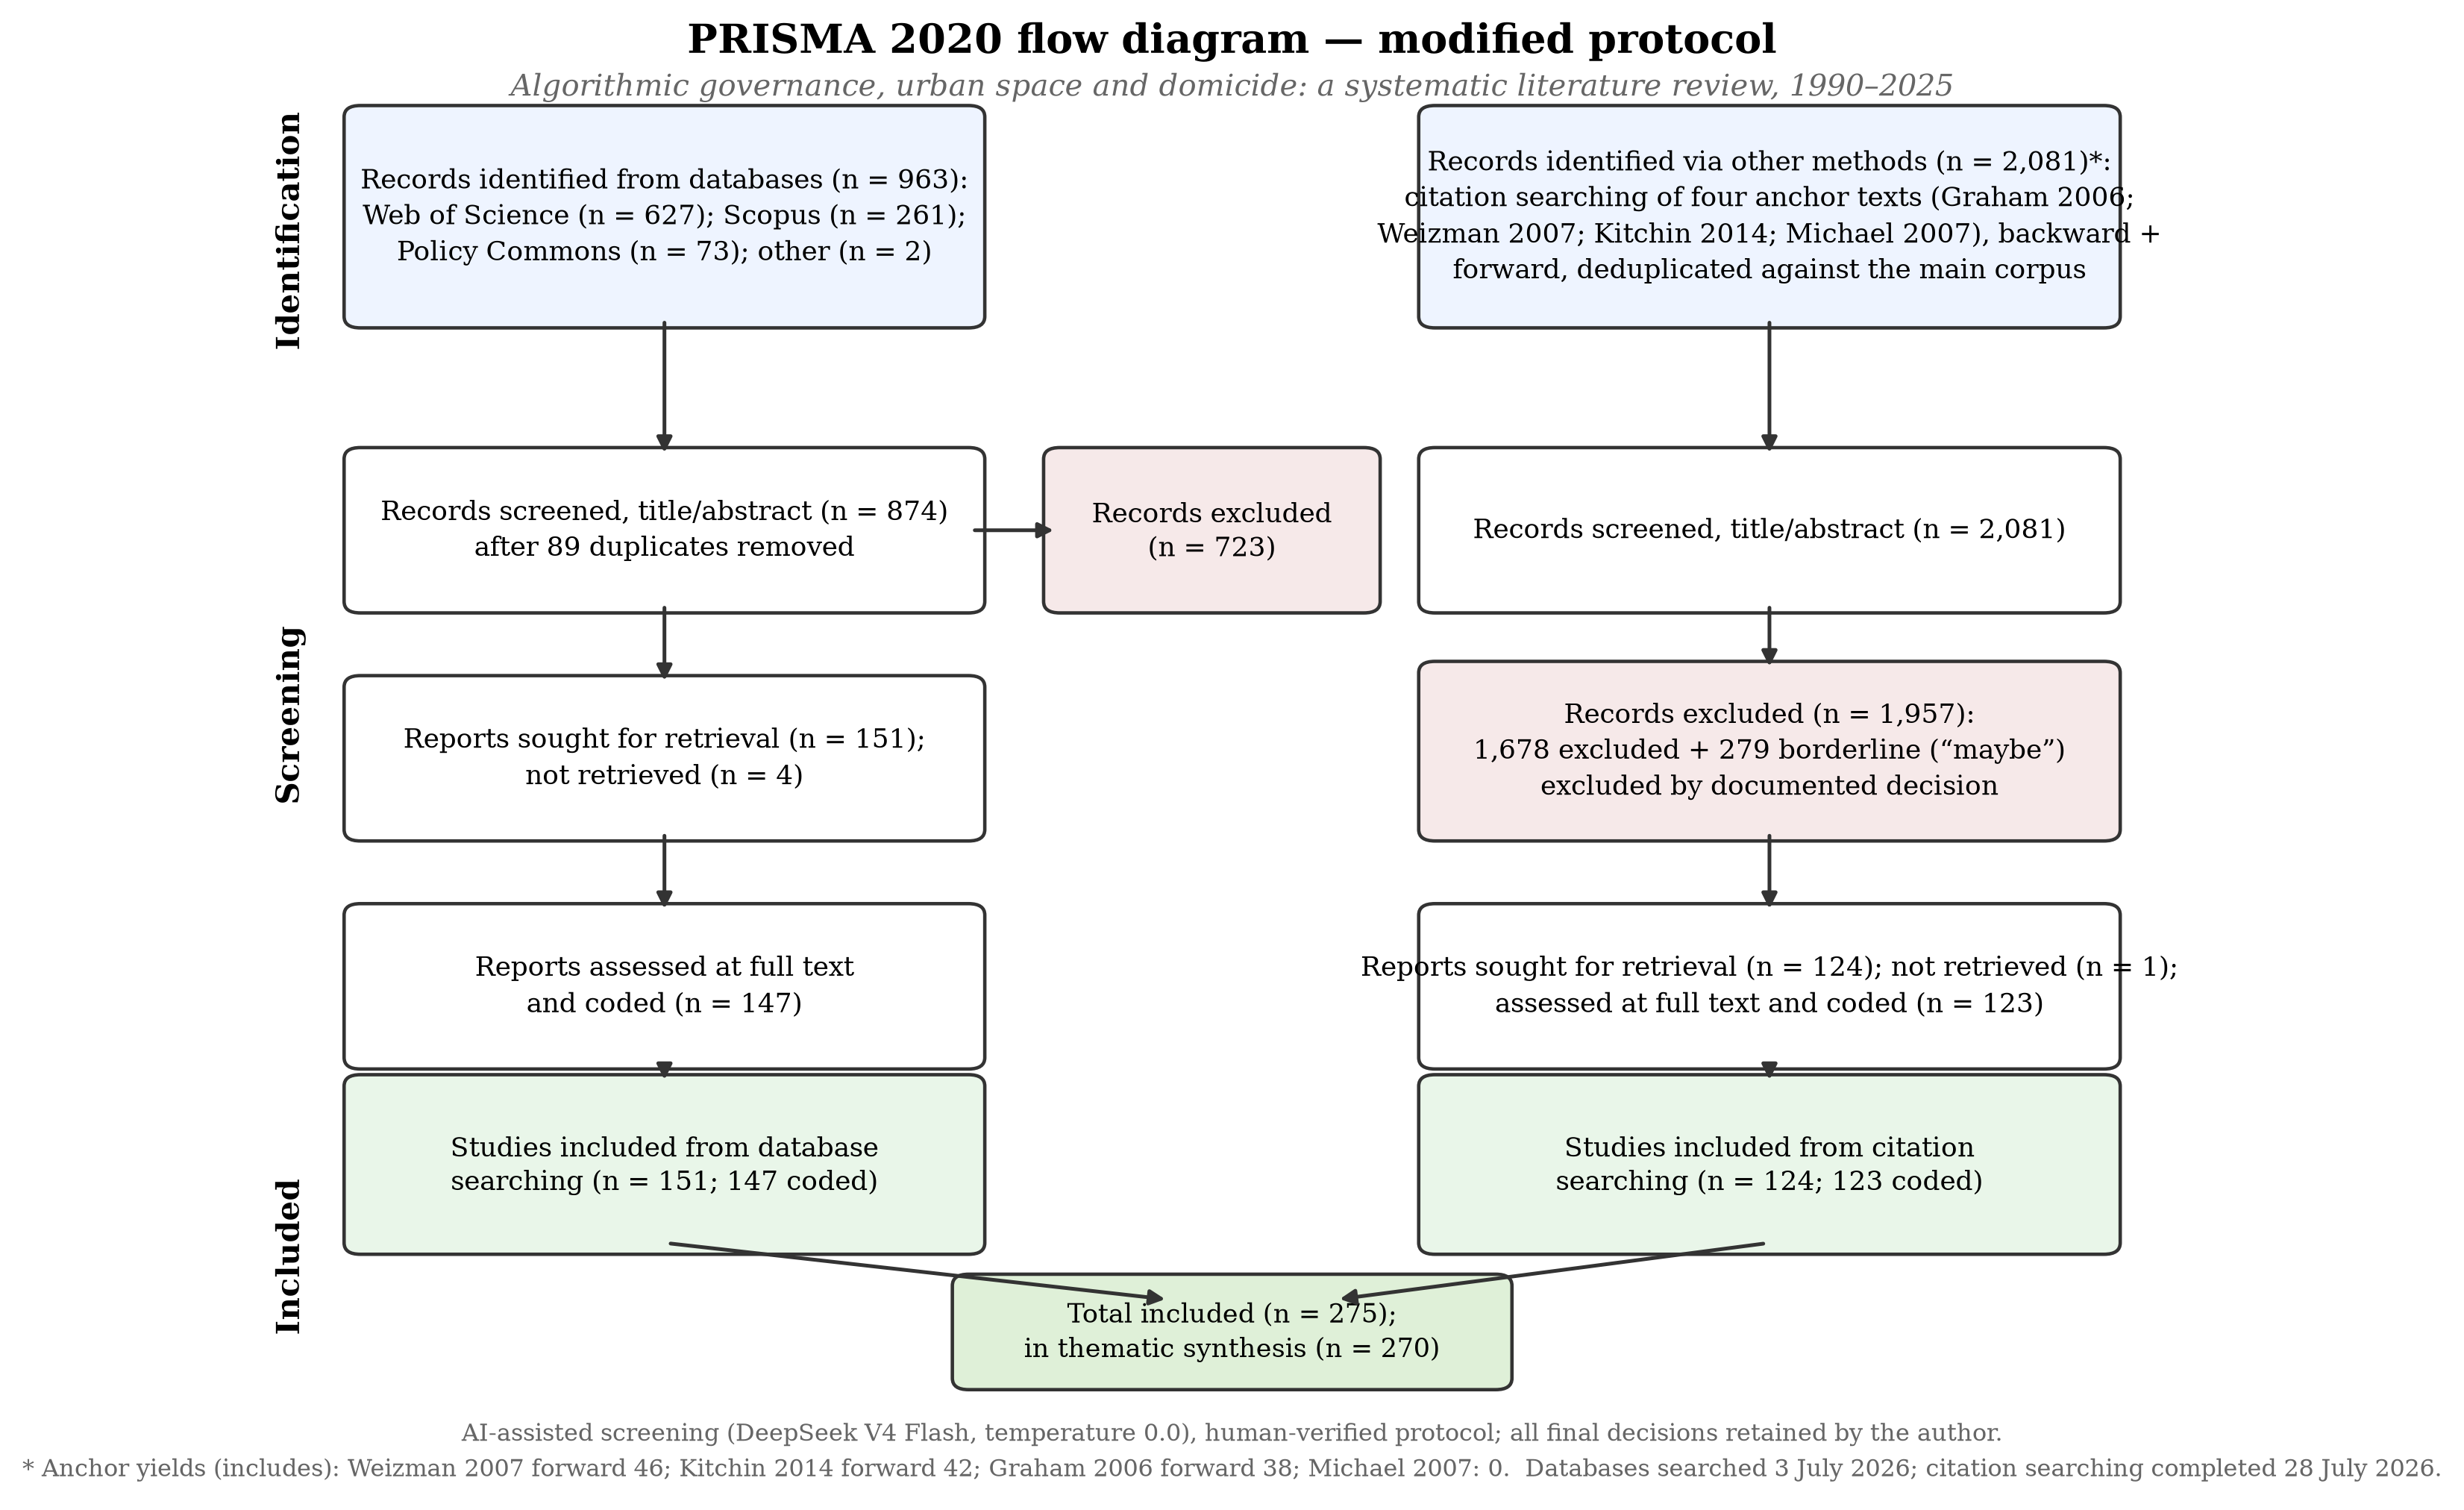
\includegraphics[width=1.16\textwidth]{figures/fig_3_1_prisma_flow_landscape.png}}
\caption{PRISMA 2020 flow diagram for the modified protocol. Final counts as of 28 July 2026: 874 unique records screened from database searches and 2,081 deduplicated citation-chaining candidates, yielding 275 included studies (270 coded).}
\label{fig:prisma}
\end{figure}